% !TeX spellcheck = en_US
\subsection{Undrained strength ratio}
\label{sec:undrained_strength_ratio}

In this example a 2D slope model is configured to setting up an undrained strength ratio of $S_u/\sigma_v=0.001$.
First, an initial simulation is performed with elastic parameters and kinetic damping for steady state condition, and then the stress field was saved with the command \texttt{"save\_state":true}. Secondly, the stress field is loaded by \texttt{"load\_state":true} and the undrained strength ratio is setting up using \texttt{"su\_vertical\_stress":0.001}.

\begin{figure}[H]
	\centering
	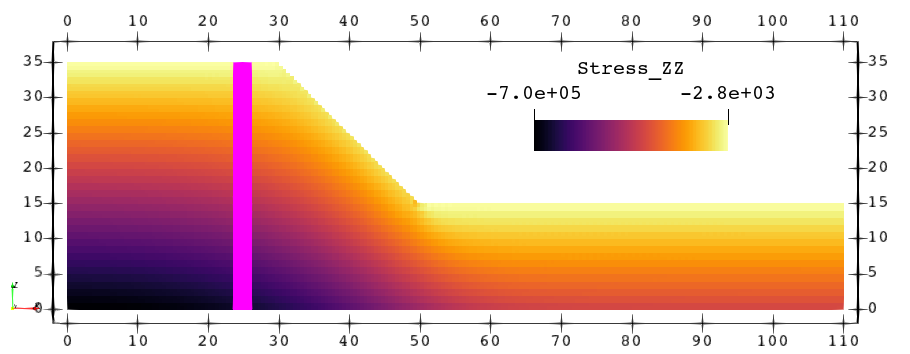
\includegraphics[width=0.7\linewidth]{../../examples/undrained-strength-vertical-stress-factor/initial-elastic-stress-field}
	\caption{Elastic stress field}
	\label{fig:initial-elastic-stress-field}
\end{figure}


\begin{figure}[H]
	\centering
	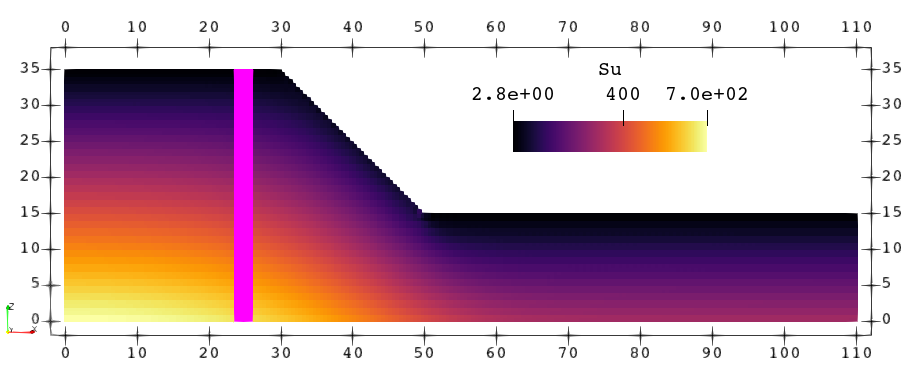
\includegraphics[width=0.7\linewidth]{../../examples/undrained-strength-vertical-stress-factor/su-factor-initial-step}
	\caption{Su factor obtained from initial stress field}
	\label{fig:su-factor-initial-step}
\end{figure}


\begin{figure}[H]
	\centering
	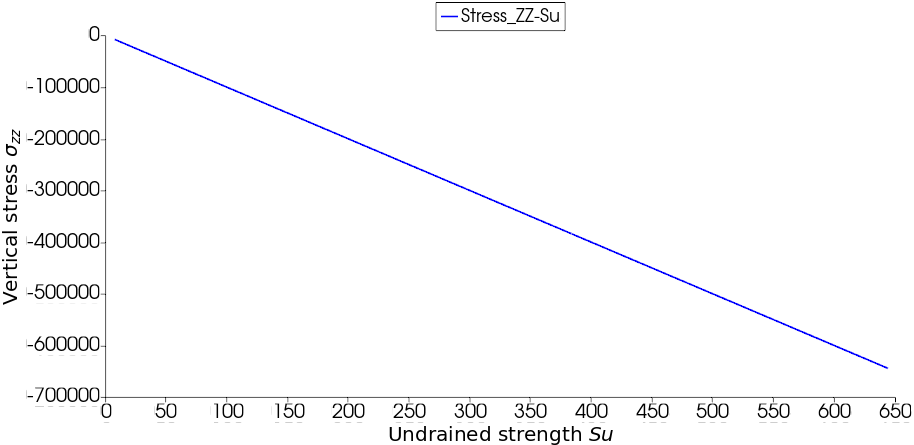
\includegraphics[width=0.7\linewidth]{../../examples/undrained-strength-vertical-stress-factor/SUu-SigmaZZ-vertical-box}
	\caption{Stress Su relation along the vertical plane defined by colored particles}
	\label{fig:suu-sigmazz-vertical-box}
\end{figure}
